
\section{Der erste Schritt}
\label{section:erste_schritte}
\begin{frame}%STARTCONTENT

\frametitle{Der erste Schritt}
\begin{columns}
    \begin{column}{0.48\textwidth}
    
\begin{figure}
    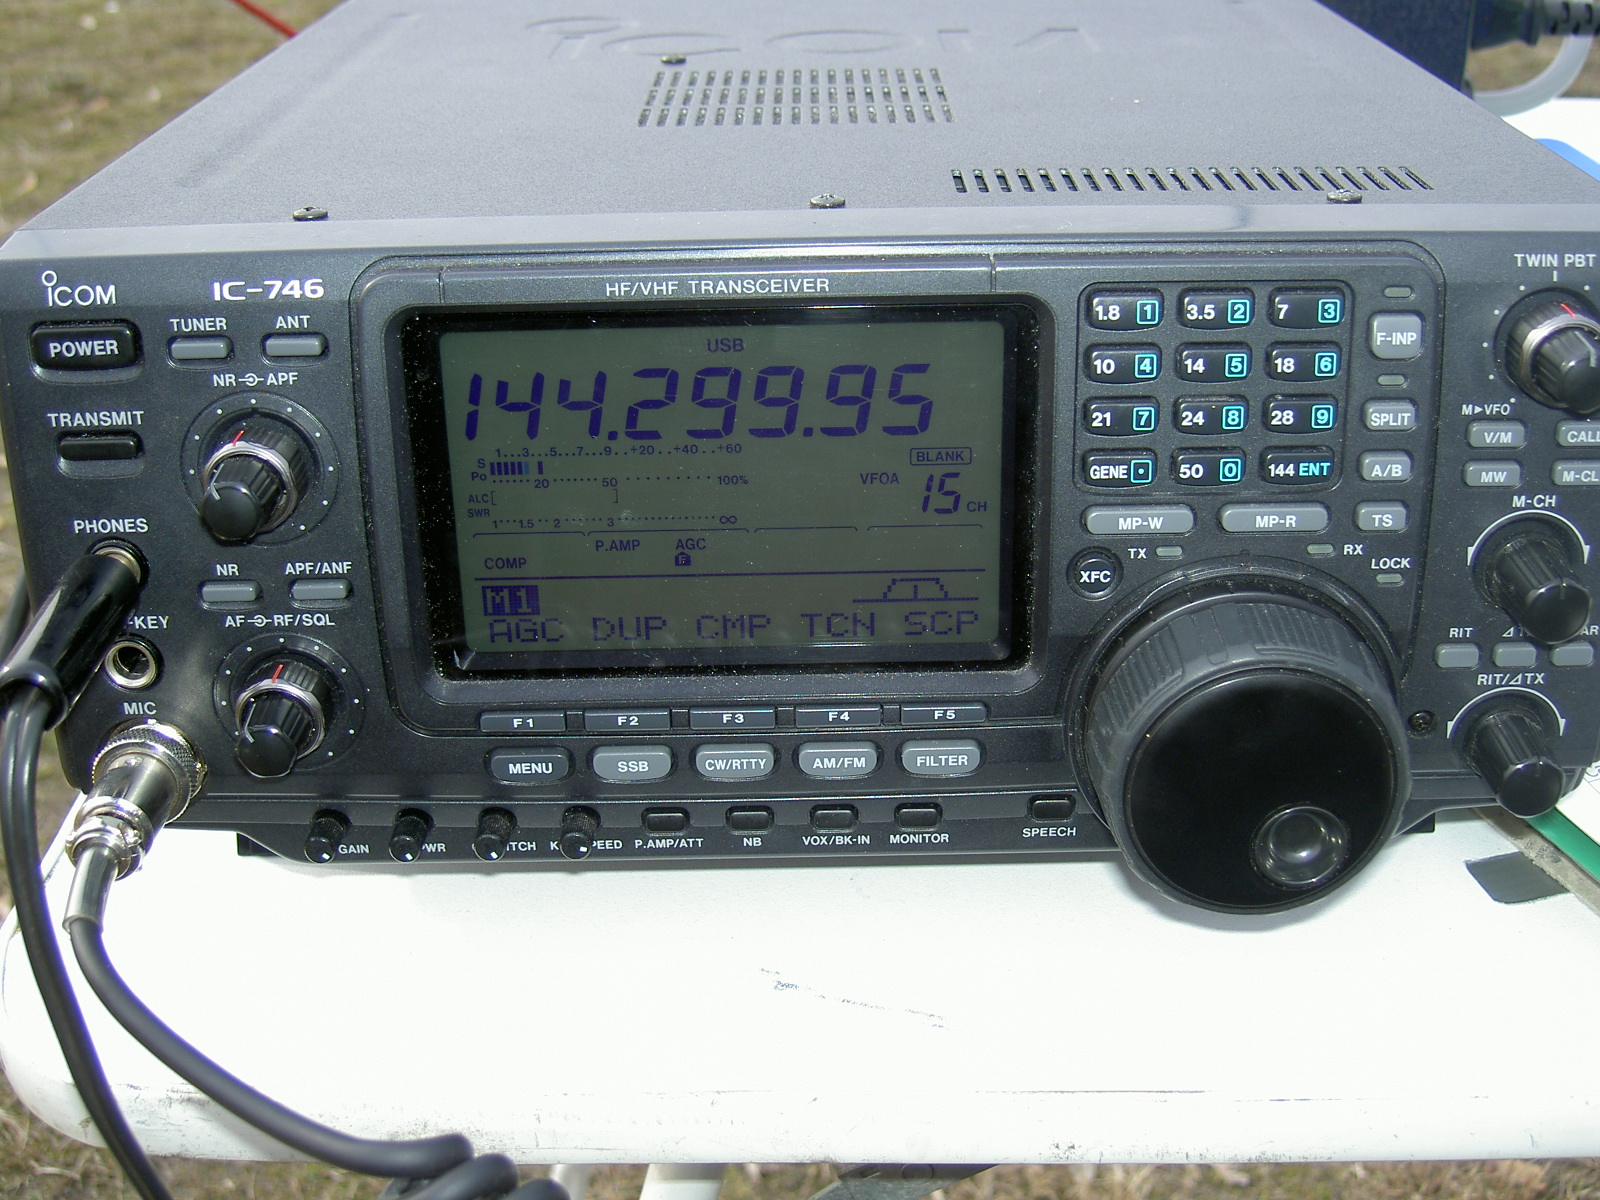
\includegraphics[width=0.85\textwidth]{foto/117}
    \caption{\scriptsize Ein Transceiver (Funkgerät) für den Amateurfunk}
    \label{n_erste_schritte_transceiver}
\end{figure}

    \end{column}
   \begin{column}{0.48\textwidth}
       \begin{itemize}
  \item Jeder darf Funkgeräte kaufen und besitzen
  \item und Amateurfunksendungen empfangen
  \end{itemize}

   \end{column}
\end{columns}

\end{frame}

\begin{frame}
\only<1>{
\begin{QQuestion}{VD102}{Was gilt in Bezug auf den Empfang von Amateurfunkaussendungen?}{Die Anerkennung als \glqq SWL\grqq{} ist erforderlich in Verbindung mit der Mitgliedschaft in einer Amateurfunkvereinigung.}
{Es dürfen nur TKG-zugelassene Empfangsgeräte verwendet werden.}
{Es bedarf der Zuteilung eines Hörerrufzeichens aus der \glqq DE-Reihe\grqq{}.}
{Es ist keine Zulassung zur Teilnahme am Amateurfunkdienst erforderlich.}
\end{QQuestion}

}
\only<2>{
\begin{QQuestion}{VD102}{Was gilt in Bezug auf den Empfang von Amateurfunkaussendungen?}{Die Anerkennung als \glqq SWL\grqq{} ist erforderlich in Verbindung mit der Mitgliedschaft in einer Amateurfunkvereinigung.}
{Es dürfen nur TKG-zugelassene Empfangsgeräte verwendet werden.}
{Es bedarf der Zuteilung eines Hörerrufzeichens aus der \glqq DE-Reihe\grqq{}.}
{\textbf{\textcolor{DARCgreen}{Es ist keine Zulassung zur Teilnahme am Amateurfunkdienst erforderlich.}}}
\end{QQuestion}

}
\end{frame}

\begin{frame}
\frametitle{Ein Funkamateur darf senden}
\begin{columns}
    \begin{column}{0.48\textwidth}
    
\begin{figure}
    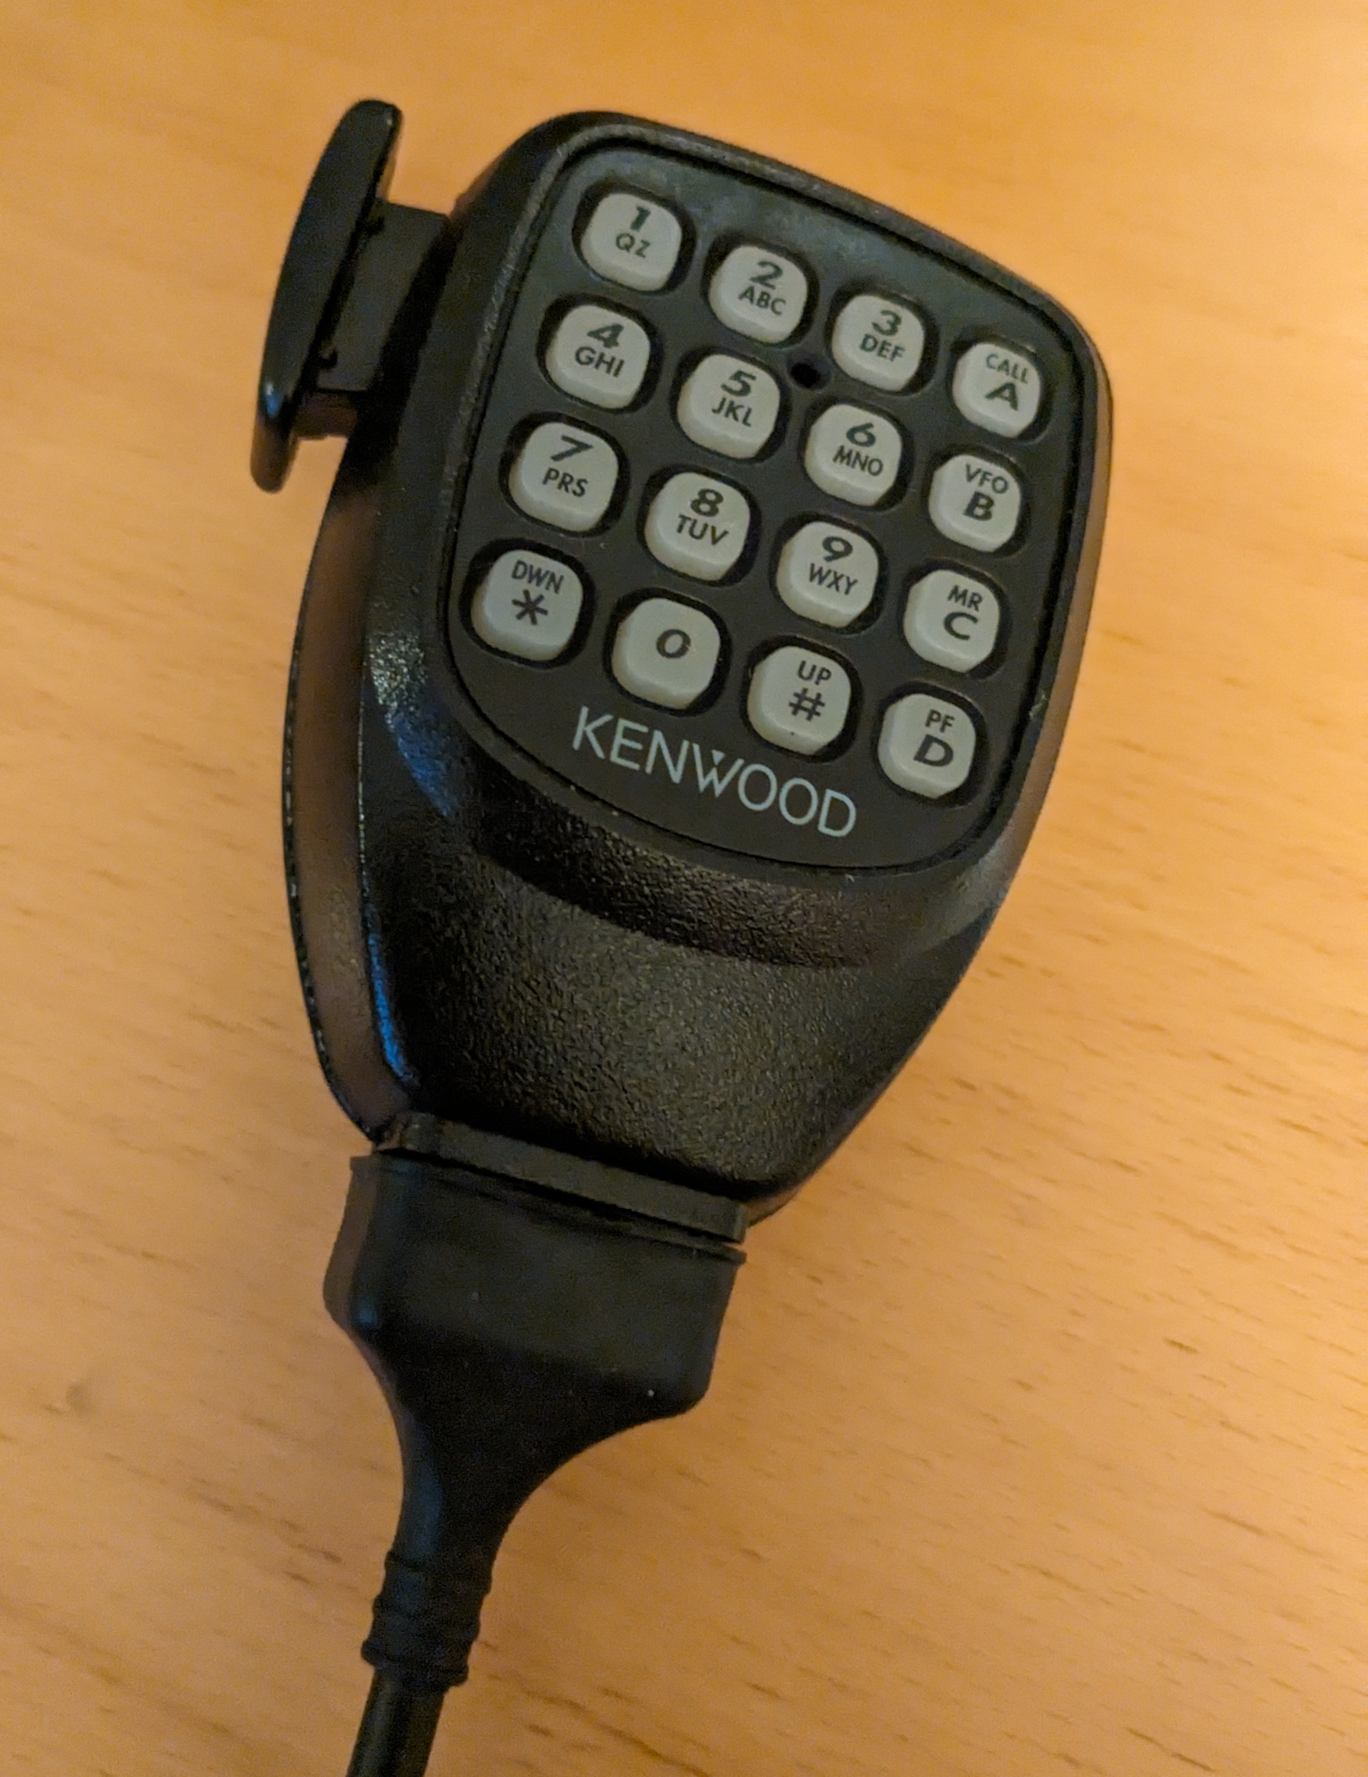
\includegraphics[width=0.85\textwidth]{foto/118}
    \caption{\scriptsize Handmikrofon mit PTT-Taste (links oben)}
    \label{n_erste_schritte_ptt}
\end{figure}

    \end{column}
   \begin{column}{0.48\textwidth}
       Auf Sendung gehen (die PTT-Taste drücken)

\begin{itemize}
  \item Taste am Funkgerät oder Mikrofon
  \item Schaltet den Transceiver von Empfangs- auf Sendebetrieb um
  \end{itemize}

   \end{column}
\end{columns}

\end{frame}

\begin{frame}
\only<1>{
\begin{QQuestion}{NF108}{Wie wird die Taste am Mikrofon bezeichnet, mit der man einen Transceiver auf Sendung schalten kann?}{RIT}
{VOX}
{PTT}
{SSB}
\end{QQuestion}

}
\only<2>{
\begin{QQuestion}{NF108}{Wie wird die Taste am Mikrofon bezeichnet, mit der man einen Transceiver auf Sendung schalten kann?}{RIT}
{VOX}
{\textbf{\textcolor{DARCgreen}{PTT}}}
{SSB}
\end{QQuestion}

}
\end{frame}

\begin{frame}
\frametitle{Mathematische Grundkenntnisse}
\begin{itemize}
  \item Im Amateurfunk werden Grundkenntnisse in Mathematik benötigt
  \item Je nach Klasse mehr Wissen notwendig
  \item Der Lehrgang unterstützt, kann aber nicht alles notwendige Wissen vermitteln
  \end{itemize}
\end{frame}

\begin{frame}
\only<1>{
\begin{QQuestion}{NA101}{Ein \qty{20}{\m} langer Draht wird bei 2/3 seiner Länge zertrennt. Wie lang sind die resultierenden Stücke in etwa?}{\qty{14,44}{\m} und \qty{5,56}{\m}}
{\qty{12,22}{\m} und \qty{7,78}{\m}}
{\qty{11,11}{\m} und \qty{8,89}{\m}}
{\qty{13,33}{\m} und \qty{6,67}{\m}}
\end{QQuestion}

}
\only<2>{
\begin{QQuestion}{NA101}{Ein \qty{20}{\m} langer Draht wird bei 2/3 seiner Länge zertrennt. Wie lang sind die resultierenden Stücke in etwa?}{\qty{14,44}{\m} und \qty{5,56}{\m}}
{\qty{12,22}{\m} und \qty{7,78}{\m}}
{\qty{11,11}{\m} und \qty{8,89}{\m}}
{\textbf{\textcolor{DARCgreen}{\qty{13,33}{\m} und \qty{6,67}{\m}}}}
\end{QQuestion}

}
\end{frame}

\begin{frame}
\only<1>{
\begin{QQuestion}{NA103}{Laut Datenblatt wiegen \qty{100}{\m} eines bestimmten Drahtes 210~g. Ein vorliegendes Drahtstück desselben Materials wiegt 55~g. Wie lang ist das Drahtstück in etwa?}{\qty{38,2}{\m}}
{\qty{382}{\m}}
{\qty{115}{\m}}
{\qty{26,2}{\m}}
\end{QQuestion}

}
\only<2>{
\begin{QQuestion}{NA103}{Laut Datenblatt wiegen \qty{100}{\m} eines bestimmten Drahtes 210~g. Ein vorliegendes Drahtstück desselben Materials wiegt 55~g. Wie lang ist das Drahtstück in etwa?}{\qty{38,2}{\m}}
{\qty{382}{\m}}
{\qty{115}{\m}}
{\textbf{\textcolor{DARCgreen}{\qty{26,2}{\m}}}}
\end{QQuestion}

}
\end{frame}

\begin{frame}
\only<1>{
\begin{QQuestion}{NA102}{Aus \qty{250}{\m} Draht sollen Antennen hergestellt werden. Pro Antenne werden \qty{18,5}{\m} benötigt. Wie viele Antennen können maximal aus dem vorhandenen Draht hergestellt werden?}{13}
{14}
{12}
{15}
\end{QQuestion}

}
\only<2>{
\begin{QQuestion}{NA102}{Aus \qty{250}{\m} Draht sollen Antennen hergestellt werden. Pro Antenne werden \qty{18,5}{\m} benötigt. Wie viele Antennen können maximal aus dem vorhandenen Draht hergestellt werden?}{\textbf{\textcolor{DARCgreen}{13}}}
{14}
{12}
{15}
\end{QQuestion}

}
\end{frame}%ENDCONTENT
